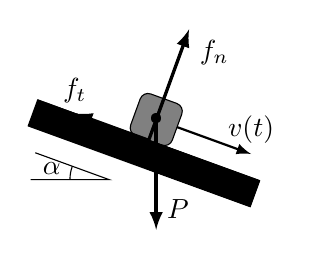
\begin{tikzpicture}[
	scale=1,
	force/.style={->,>=latex,draw=\JRLblue,very thick,nodes={\JRLblue}},
	plane/.style={draw=\JRLblueC,fill=\JRLblueC},
	vecteur/.style={-latex,thick},
	]
	% bloc
	\draw[fill=gray,rounded corners=3pt,rotate=-20] (-8pt,0) rectangle (8pt,16pt);
	% support
	\draw[plane,rotate=-20](-1.5,0)rectangle(1.5,-10pt);
	\draw[\JRLblueF,rotate=-20](-1.5,0)--(1.5,0);
	% angle
	\draw[shift={(-.5,-.5)}](-1,0)--++(1,0)--++(160:1);
	\draw[shift={(-.5,-.5)}](-.5,0)arc(180:160:.5);
	\draw[shift={(-.5,-.5)}](170:.5)node[left, yshift=0.5mm]{$\alpha$};
	% vitesse
	\draw[vecteur,rotate=-20](8pt,8pt)--++(1,0)node[above]{$\vv{v}(t)$};
	% forces
	\draw[force,rotate=-20](0,0)--++(-1,0)node[above]{$\vv{f_\text{t}}$};
	\draw[force,rotate=-20](0,0)--++(0,1.5)node[below right]{$\vv{f_\text{n}}$};
	\draw[force](2.7pt,7.5pt)node{•}--++(0,-1.4)node[above right]{$\vv{P}$};
\end{tikzpicture} 